\section{Introduction}
With the development of AI technology, many work are done by robot instead of human. Driving is one of these tasks and autonomous driving(AD) has become more and more popular these years. It's obvious that AD technology will be one of the hottest topics of AI. The reason why this topic is so hot is that AD is not one single technology, but rather a highly complex system that consists of many sub-systems\cite{liu2017creating}. Nowadays, a well-performed AD car usually has multiple sensors like GPS, lidar and camera to perceive the world around it. The huge amount of sensing data generated is transferred into the computer to do processing, then the location and some other information are calculated to help the car makes decisions all by itself. AD is the area where any researcher is able to find their research interests and make contributions.

\begin{figure}[t]
    \centering
    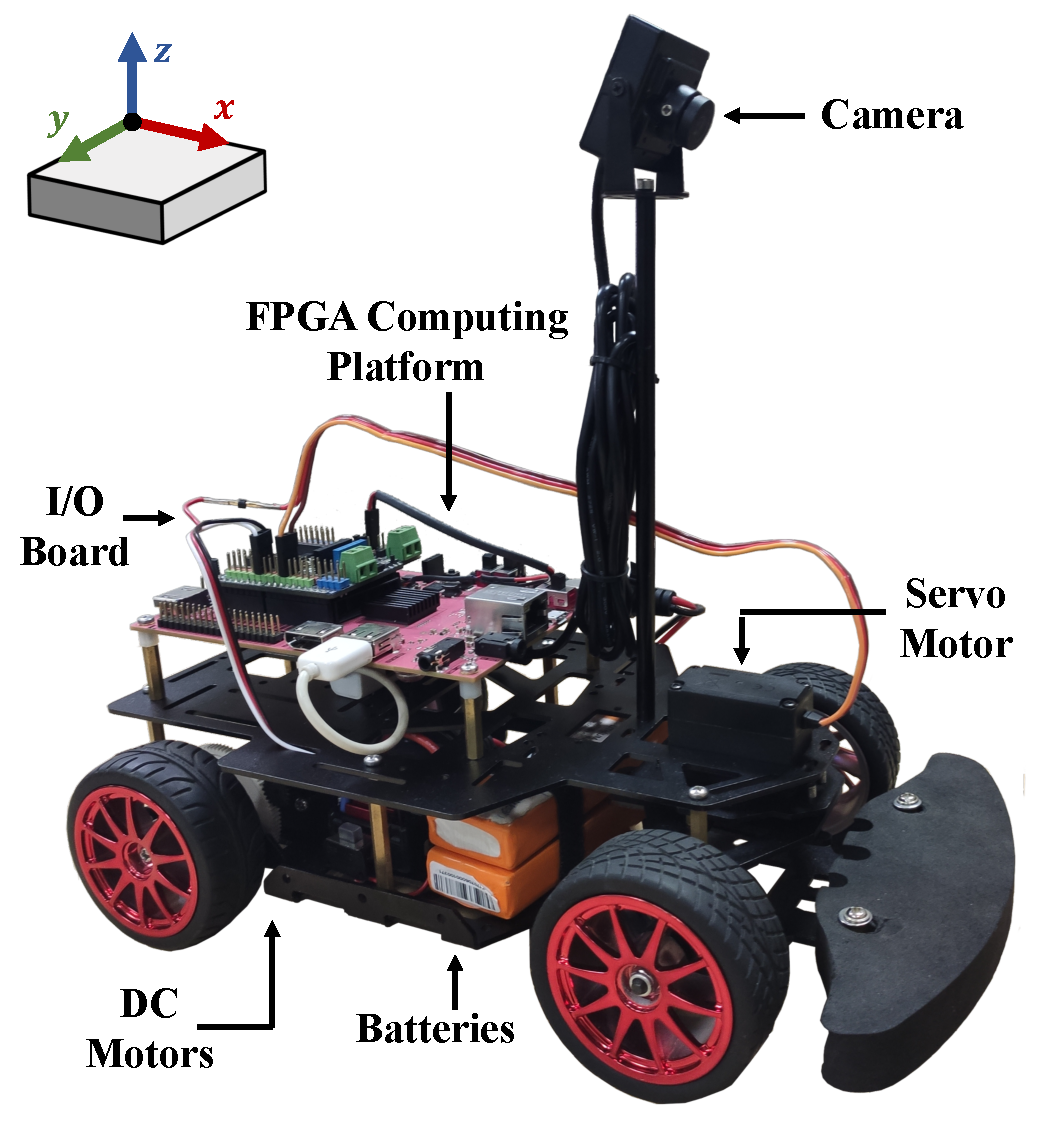
\includegraphics[width=2.5in]{hydramini}
    \caption{Overview of HydraMini Platform.}
    \label{fig:hydramini}
\end{figure}

Since there will be more people trying to learn about AD technology, a platform for AD researching and learning is badly needed. As we all know that in the cloud computing domain, researchers usually want to own machines that have good computation performance. The data center based on virtualization technology\cite{nurmi2009eucalyptus} and distributed computing\cite{dean2008mapreduce} nowadays usually has many powerful servers for data processing. And for AD tasks which are usually run in edge side, the importance of good performance is just the same as in cloud computing. The acceleration of the inference process through hardware is becoming more and more common and indispensable, it's the cornerstone of the development of AD and all the researchers and students should pay enough attention to it. However, when it comes to edge computing\cite{shi2016edge}, we should care about not only the computing power but also the power consumption and cost. It's a pity that we can hardly find one product that provides both enough computing power and hardware acceleration but remains affordable for most of the people.

\begin{table*}[t]
\centering
\caption{Platform Comparison.}
\label{tab:comparision}
\begin{tabular}{l|cccc} 
\hline
Features & Donkey Car & F1/10 & HydraOne & HydraMini \\ \hline
\hline
Computing Board & Raspberry Pi & NVIDIA Jetson TX1/TX2 & NVIDIA Jetson TX2 & Xilinx PYNQ-Z2 \\
Compputing Architecture & CPU & CPU + GPU & CPU + GPU & CPU + FPGA \\
Camera & Monocular $\times 1$ & Monocular $\times 1$ + Deep $\times 1$ & Monocular $\times 2$ & Monocular $\times 1$ \\
LiDAR & - & 2D LiDAR $\times 1$ & 3D LiDAR (16 Laser Units) $\times 1$ & - \\
Resource Management Model & - & Publisher/Subscriber (ROS) & Publisher/Subscriber (ROS) & Producer/Consumer \\
Typical Cost & $\sim\$200$ & $\sim\$2,400$ & $\sim\$1,500$ (w/o LiDAR) & $\sim\$200$ \\ \hline
\end{tabular}
\end{table*}

To make everyone have the opportunity to participate in the research of AD, we propose HydraMini, an affordable indoor experimental research and education platform for AD. It's concise and powerful, users could both learn easily and have an in-depth study. The platform was first designed for the design competition of FPT 2019\cite{wu2019end}, in this competition competitors need to build an AD car which has the abilities to finish common tasks in AD area like run along the road, avoid obstacles, understand meanings of traffic lights and so on. After attending the competition, we find the potential of our design and decide to make the project a common platform for researchers and students. As shown in Fig.~\ref{fig:hydramini}, HydraMini is a powerful and flexible platform from hardware to software. It depends on three main components: mechanical component, control system and FPGA accelerator which are the basic of modern AD technology.

We have built several study cases based on HydraMini, people are able to try AD car in a traditional way which uses computer vision methods to follow the road and do some pattern recognition, or they apply an end-to-end AI model to generate control commands directly. Also we accelerate the inference process of YoloV3\cite{redmon2018yolov3} and make it fast enough to work in a limited edge device. What's more, if your research project is based on  ROS\cite{quigley2009ros} which is widely used in robots all over the world, the migration of your project to HydraMini is easy, and with the support of functions of our platform you will probably come up with more exciting ideas. Besides, we provide tools for users, one of them is a simulator using Unity3d\cite{2019unity3d} based on sdsandbox\cite{sdsandbox} that makes the users test their design more conveniently. All the resources on HydraMini are managed by PYNQ-Z2\cite{tul2019tulpynqz2} system which is based on Ubuntu 18.04. 

Users use the computing power in PYNQ-Z2 includes both Zynq7020 FPGA\cite{zynq} which is used as a specialized hardware accelerator and an Arm 32-bit core ARM Cortex-A9 which is familiar to normal people. We believe that in the future the hardware acceleration will become an imperative for the modern cars to provide edge computing power, so it's necessary to embed FPGA which is flexible for researching in our platform. Users will find it easy to do research on multi-area of AD and develop their own algorithms and systems based on HydraMini.

The remainder of this paper is organized as follows. In Section Ⅱ, we discuss the related work. Section Ⅲ introduces the design and implementation details of HydraMini. In Section Ⅳ, we summarizes three key characteristics of our platform. We provide several case studies to show the large potential of HydraMini in Section Ⅴ. Finally, we conclude our work in Section Ⅵ.